\documentclass[a4paper]{article}

\usepackage[utf8]{inputenc}
\usepackage[T1]{fontenc}
\usepackage{textcomp}
\usepackage[dutch]{babel}
\usepackage{amsmath, amssymb}
\usepackage{code}
\usepackage{pythonhighlight}

% figure support
\usepackage{import}
\usepackage{xifthen}
\pdfminorversion=7
\usepackage{pdfpages}
\usepackage{transparent}
\usepackage{graphicx}
\pdfsuppresswarningpagegroup=1
\graphicspath{{./img/}}
\begin{document}
\section{Intro - lightboard}
Everything follows right hand rule
\begin{figure}[htpb]
	\centering
	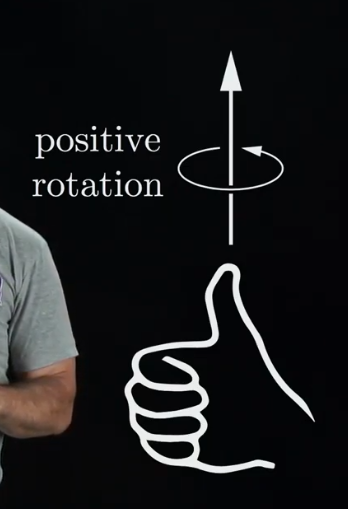
\includegraphics[width=0.5\textwidth]{postiveRotaion.png}
	\caption{}
	\label{fig:}
\end{figure}
\section{Foundation of mobile robotics ch-2}
\subsection{Degrees of freedom rigid body}
\begin{itemize}
	\item \textbf{Configuration} - A specific position of the position of all points of robot
	\item \textbf{C-space} - The space of all configuration
	\item \textbf{degrees of freedom} - dimension of c space
	\item Rigid body has 6 degrees of freedom

	\item dof - $\sum (freedom points) - no.of.constrains$ \\\
                        \begin{tabular}{|c|c|c|c|}
                        \hline
                        points & dof & no.of.constrains & constrans \\
                        \hline
                        point A & 2 & 0 & - \\ 
                        point B & 2 & 1 & $d_{ab}$ \\ 
                        Point C & 2 & 2 & $d_{ac},{d_bc}$ \\
                        \hline
                        \end{tabular}
	\item $dof = m(N-1) - \sum_{i=1}^J c_i$
\end{itemize}
\subsection{Degree of freedom of a robot}
\begin{itemize}
        \item Joint - constrains the dof of rigid body
\end{itemize}
insk
\end{document}
